\section{Results and Analysis}
\label{sec:results}

All results are computed from the six trial CSV files in \path{results/raw/} using the analysis script \path{analysis/plot.py}. Unless stated otherwise, each value is the mean over three runs, with one sample standard deviation. Lower values are better for latency, scale-up time, and drain time; lower final pod counts are better after the workload has stopped.

\subsection{Headline Metrics}
\label{subsec:res-summary}
Table~\ref{tab:summary} shows the aggregate results. KEDA wins on all responsiveness metrics and is the only strategy that releases capacity before the observation window ends. The two strategies reach the same peak of six pods, so the difference is not maximum capacity. The difference is how early each strategy receives useful information about the burst and about the remaining backlog.

\begin{table}[t]
  \centering
  \small
  \caption{Headline metrics per strategy (mean $\pm$ standard deviation, $n=3$). ``---'' means the event was not observed within the trial window.}
  \label{tab:summary}
  \begin{tabular}{lcc}
    \toprule
    \textbf{Metric} & \textbf{HPA: CPU signal} & \textbf{KEDA: queue signal} \\
    \midrule
    \multicolumn{3}{l}{\emph{Responsiveness}} \\
    Reaction latency (s)                  & $73.8 \pm 8.3$   & $\mathbf{63.4 \pm 3.4}$ \\
    Time to peak pods (s)                 & $90.2 \pm 4.6$   & $\mathbf{80.2 \pm 5.1}$ \\
    Queue drain time (s)                  & $309.7 \pm 5.2$  & $\mathbf{297.6 \pm 5.6}$ \\
    \midrule
    \multicolumn{3}{l}{\emph{User-visible effect}} \\
    Avg. throughput during drain (msg/s)  & $22.75 \pm 0.27$ & $\mathbf{23.35 \pm 0.27}$ \\
    Messages delivered per trial          & $7\,451 \pm 57$  & $7\,212 \pm 90$ \\
    \midrule
    \multicolumn{3}{l}{\emph{Resource use}} \\
    First scale-down (s after burst end)  & ---              & $\mathbf{326.9 \pm 3.1}$ \\
    Ready pods at trial end               & $6.0$            & $\mathbf{3.0}$ \\
    Pod-seconds overshoot                 & $1\,426 \pm 27$  & $\mathbf{1\,415 \pm 7}$ \\
    Peak pod count                        & $6$              & $6$ \\
    \bottomrule
  \end{tabular}
\end{table}

The total delivered-message count should be interpreted as descriptive rather than as a direct performance score, because the actual number of messages published varies slightly with producer-side timing. Queue-drain time and delivery throughput are more comparable across runs because they normalize behaviour over the observed drain period.

\subsection{Responsiveness}
\label{subsec:res-response}
Fig.~\ref{fig:response} visualizes the three latency-style metrics. Compared with the CPU-based HPA, KEDA reacts 10.4~s earlier on average, which is a 14\% reduction in reaction latency. It also reaches the maximum useful replica count about 10~s earlier and clears the queue 12.2~s earlier. These differences are operationally meaningful: in a queue-backed service, every second of delayed scale-out allows the backlog to grow further.

\begin{figure}[t]
  \centering
  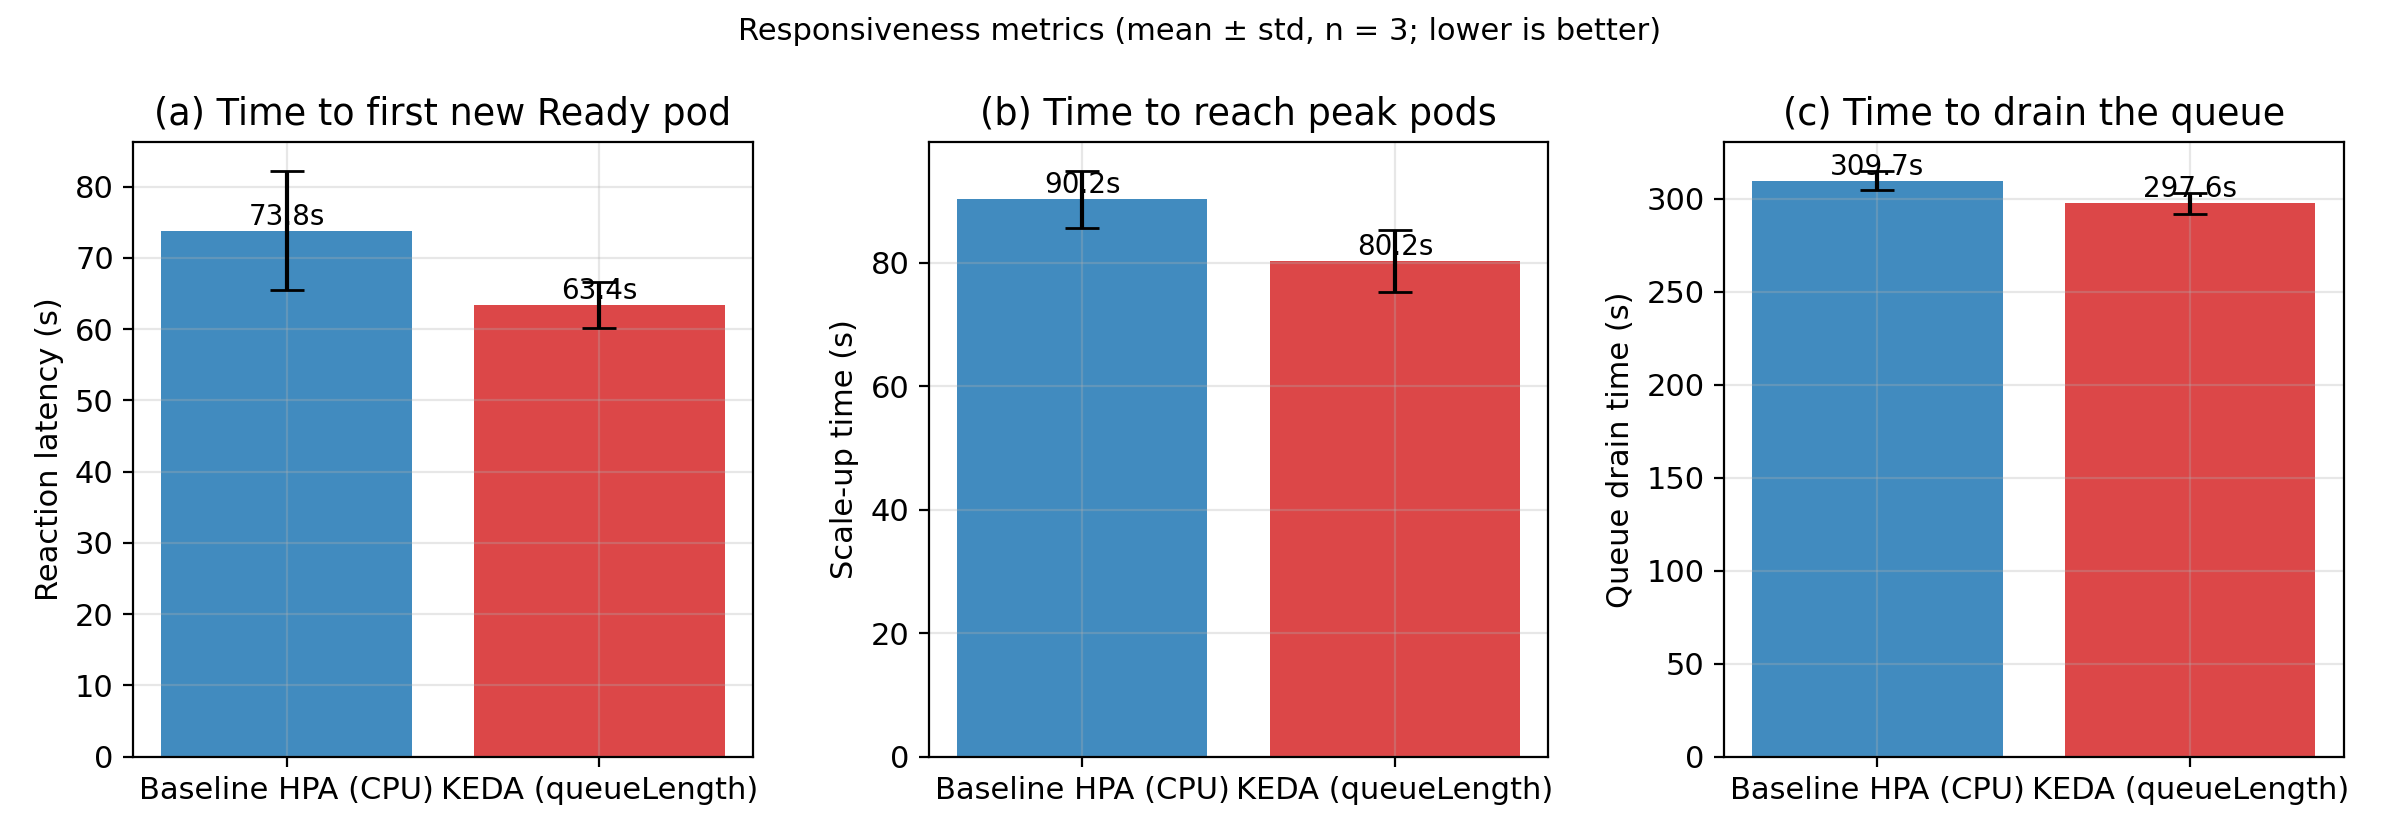
\includegraphics[width=0.93\linewidth]{../results/figures/fig4-response-bar.png}
  \caption{Responsiveness metrics. KEDA responds earlier because queue length is visible as soon as backlog forms, while CPU-based HPA waits for resource metrics to cross the target.}
  \label{fig:response}
\end{figure}

The per-run timeline figures in \texttt{results/figures/} show the same pattern in every matched run. KEDA reaches 5--6 Ready pods first, its queue-depth curve stays below the baseline HPA during the drain, and only KEDA removes pods before the trial ends. The aggregate bar chart therefore reflects a consistent run-level pattern rather than a single outlier.

\subsection{Scale-down Behaviour}
\label{subsec:res-scaledown}
The strongest qualitative difference appears after the burst stops. Fig.~\ref{fig:scaledown} shows that the baseline HPA does not scale down in any trial, while KEDA starts removing pods about 327~s after the burst ends and reaches three Ready pods by the end of the observation window. This is notable because both strategies use the same 60~s scale-down stabilisation window and the same 50\%/60~s removal policy.

\begin{figure}[t]
  \centering
  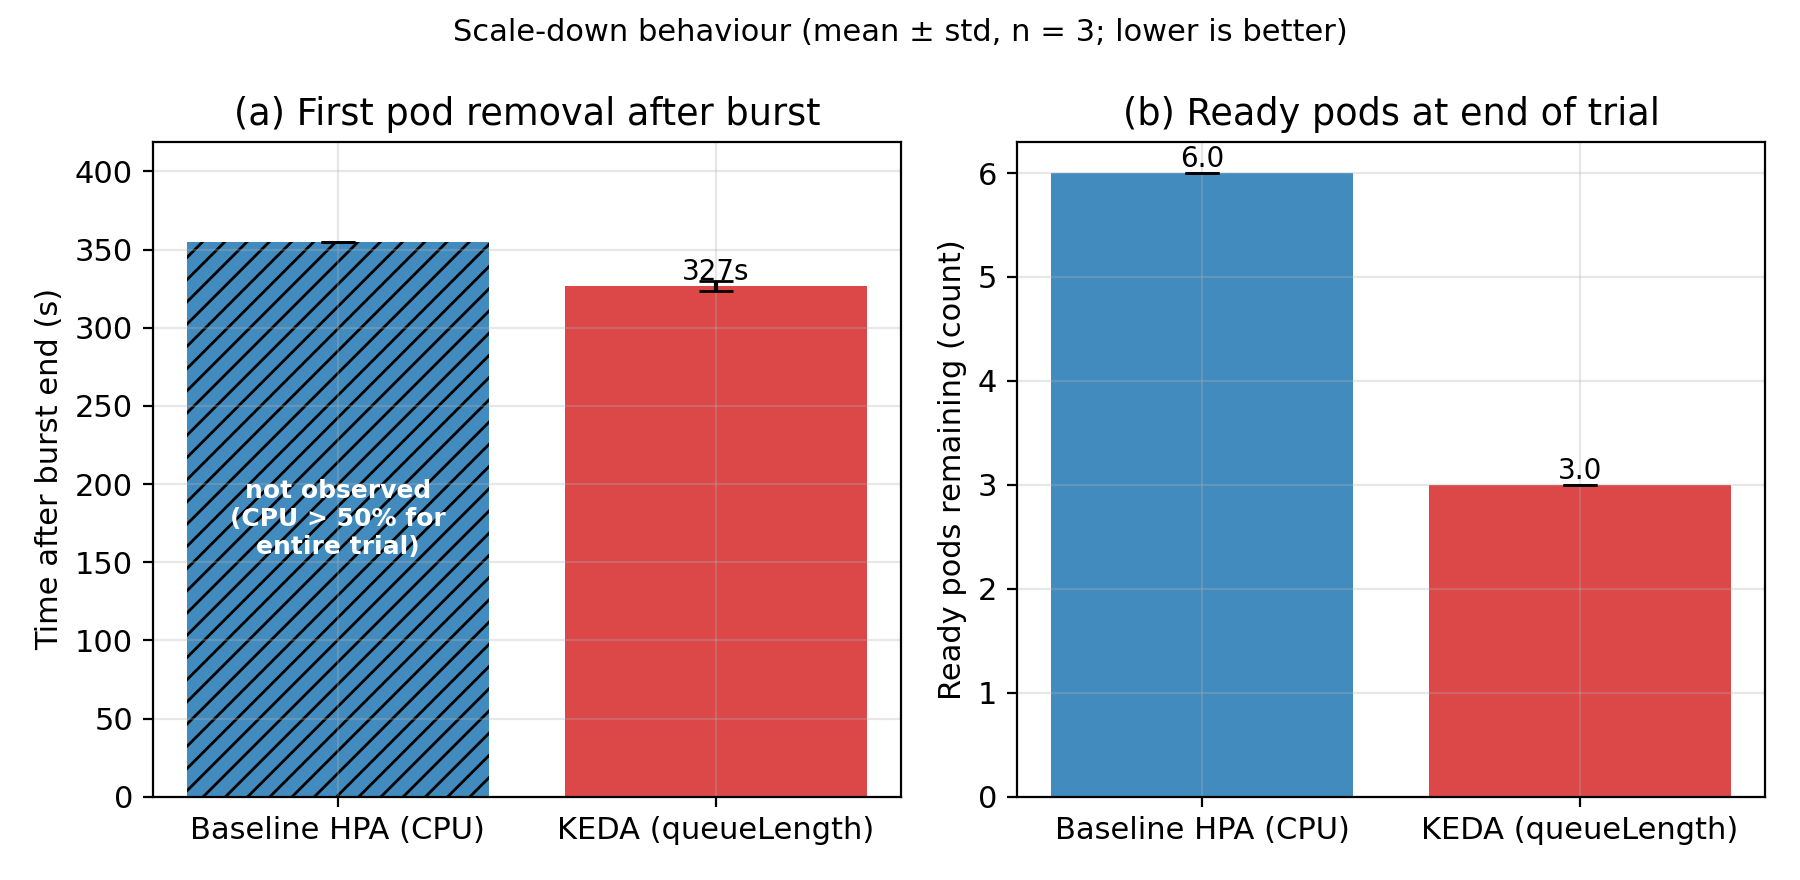
\includegraphics[width=0.93\linewidth]{../results/figures/fig5-scale-down-bar.png}
  \caption{Scale-down behaviour. The CPU-based HPA remains at six pods during the trial, while KEDA begins returning capacity once queue depth falls sufficiently.}
  \label{fig:scaledown}
\end{figure}

\textbf{Why HPA cannot shrink in the observed window.} The consumer is CPU-bound, and each pod is limited to 300~m CPU while requesting 100~m. As long as a pod has messages to process, it can remain close to the CPU limit. The HPA therefore observes utilisation near $300\%$ of the CPU request, far above the 50\% target. Substituting that ratio into Eq.~\ref{eq:hpa} keeps the desired replica count clamped at \texttt{maxReplicas}=6 until the queue is almost empty. In other words, the CPU signal tells HPA that the pods are busy, but it does not tell HPA that the backlog is already shrinking.

\textbf{Why KEDA shrinks earlier.} KEDA observes the queue directly. With the target $T=100$ messages per replica, the desired replica count decreases as $Q$ decreases. Once the queue has dropped far enough, KEDA can recommend fewer than six pods, and the shared 60~s stabilisation window delays but does not prevent the downscale. This is the key technical lesson of the experiment: using an event signal changes not only scale-up timing but also the ability to detect when extra capacity is no longer needed.

\subsection{Resource Cost Interpretation}
\label{subsec:res-cost}
The pod-seconds overshoot is similar for the two strategies: $1\,426 \pm 27$ for HPA and $1\,415 \pm 7$ for KEDA. This does not contradict the scale-down result. Both strategies quickly reach the same six-pod cap, and most of the trial is spent processing the burst, so the cost curves are similar over this short window. KEDA's cost advantage appears in the tail because it starts returning pods earlier. A longer post-drain observation period would likely enlarge the pod-seconds gap.
